\lab{Applications}{Balanced Trees}{Balanced Trees}
\label{lab:btrees}

Trees are very versatile structures.  
Their worst case complexity of $O(\log n)$ for inserting, deleting, and searching make them an attractive option when working with lots of data.
In most cases, a simple binary search tree is sufficient.
However, there are cases when we lose all the benefits of a binary search tree.
One example is adding already sorted or nearly sorted data to a binary search tree.
This results in a degnerate BST that performs no better than a linked list!
Another problem is adding more levels to the tree than is necessary.
The more levels a tree has, the less performant it becomes.  If we could somehow fill a level or make it as close to full as possible, we can minimize the number of levels a a search tree has.

\begin{problem}
Write methods to determine the number of levels a tree has and how full each level is.  Look at breadth first search for inspiration on how to accomplish this.
\end{problem}

\section*{Balancing Trees}
There have been a variety of attempts at optimizing the structure of a binary tree.
The method that we will describe in depth is and AVL balanced tree.
AVL trees use the strictest definition of balance.
Another commonly used balanced binary tree is a red-black tree.  AVL trees optimize frequent lookups while red-black trees optimize insertion/deletion performance.
Red-black trees color nodes red or black and check for imbalance based on colors.  For example, a subtree is unbalanced if a red node has a red child.
AVL trees determine balance by comparing the height of right and  left subtrees.
The height of a node is a measure of how far up the tree the node is from the base.
There are four ways a binary tree can be unbalanced in an AVL tree.

\subsection*{Left-Left and Right-Right}
\begin{figure}[h]
\centering
\begin{subfigure}[b]{.49\textwidth}
    \centering
    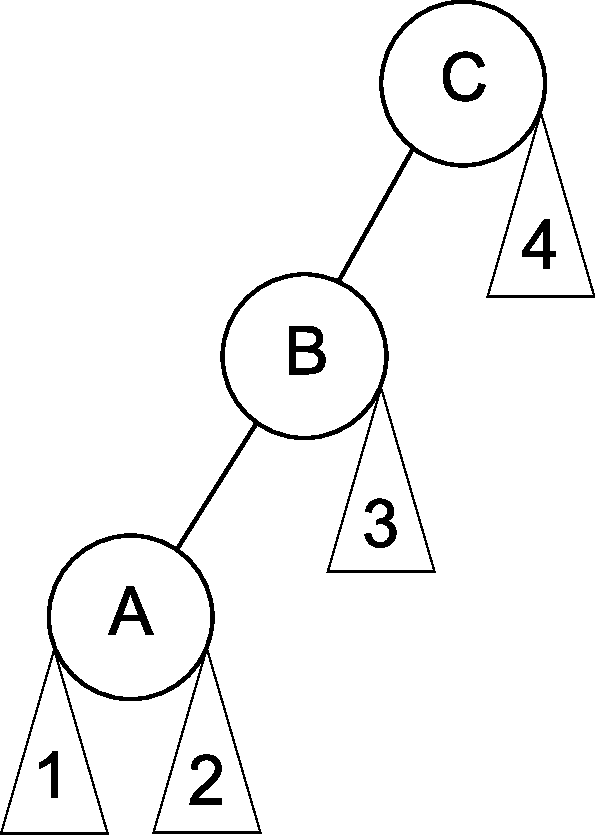
\includegraphics[width=.75\textwidth]{left_left.pdf}
\end{subfigure}
\begin{subfigure}[b]{.49\textwidth}
    \centering
    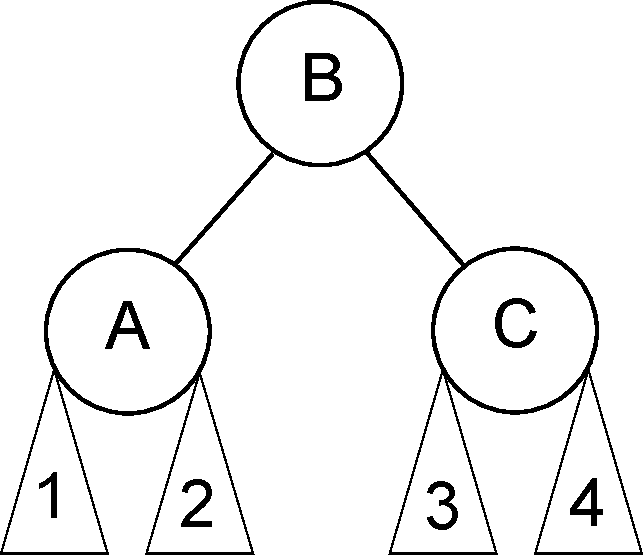
\includegraphics[width=.75\textwidth]{balanced.pdf}
\end{subfigure}
\end{figure}

One of the primary cases, this imbalance can solved by a single rotation.
This will rotate the tree so that node B is the new root of the tree.
Node C becomes a child node of B and the right subtree of node becomes a left subtree of node C.
This preserves the ordered property of the tree.

\begin{figure}[h]
\centering
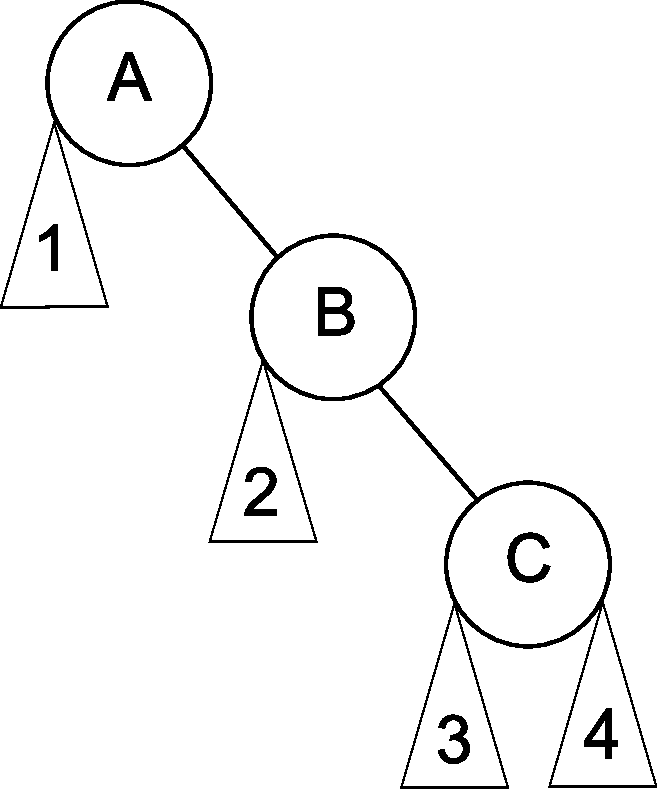
\includegraphics[width=.33\textwidth]{right_right.pdf}
\caption{The mirror image of the Left-Left case.}
\end{figure}

\subsection*{Left-Right and Right-Left}
\begin{figure}[h]
\centering
\begin{subfigure}[b]{.49\textwidth}
    \centering
    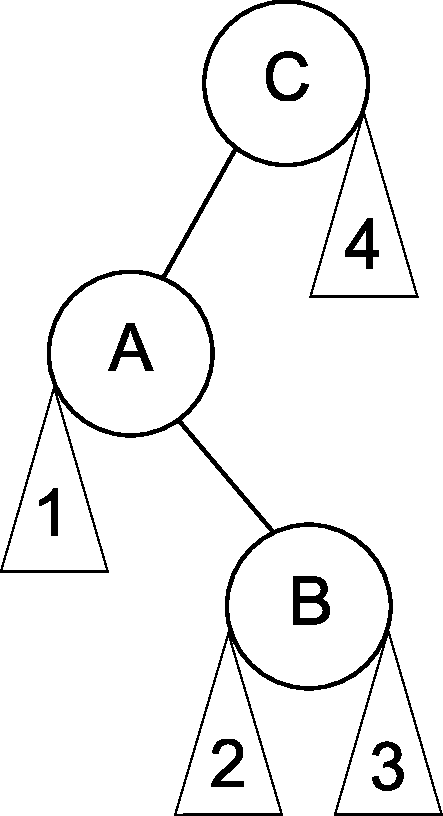
\includegraphics[width=.75\textwidth]{left_right.pdf}
\end{subfigure}
\begin{subfigure}[b]{.49\textwidth}
    \centering
    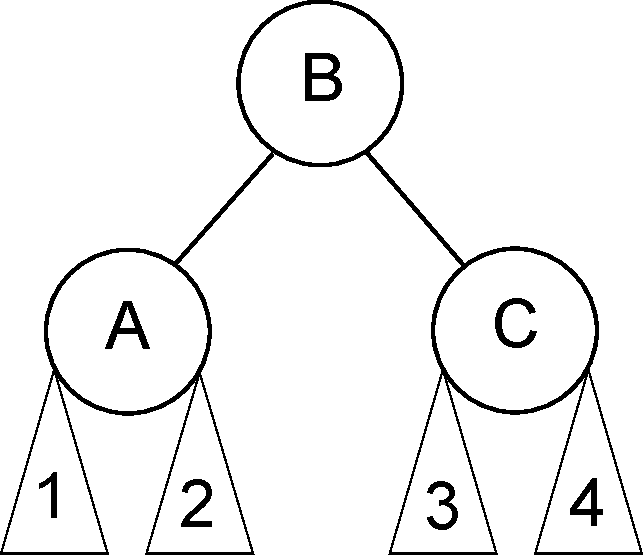
\includegraphics[width=.75\textwidth]{balanced.pdf}
\end{subfigure}
\end{figure}

These cases are a little more complex.
Two rotations must be performed to remedy the imbalance.
Node C is out of balance.
We first need rotate node B to be the parent of node A.
The left subtree of node B becomes the right subtree of node A.
Now we have to do a right rotate, moving node B to be the new root.
Node C becomes a child of node B and the the right subtree of B becomes the left subtree of node C.

\begin{figure}[h]
\centering
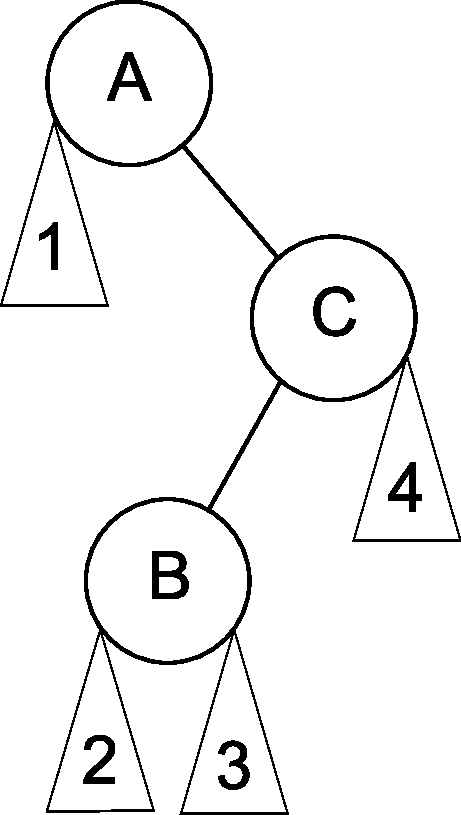
\includegraphics[width=.33\textwidth]{right_left.pdf}
\caption{The mirror image of the Left-Right case.}
\end{figure}

\begin{problem}
% TODO: Update with references to Datastructures lab.
Subclass the BST from the Data Structures lab and add methods for balancing the BST.
You will also need to override the insert and remove methods from the BST because an AVL tree must be rebalanced on each insert or removal.
\end{problem}

\section*{Balanced Trees}
